% =========================================================
% TikZ diagram: The Unifying Theorem — three-way closure equivalence
% Place: in notes-sequential-characterizations.tex
%        after the closure equivalence theorem
% Requires: \usetikzlibrary{positioning, arrows.meta}
% =========================================================

\begin{figure}[h]
\centering
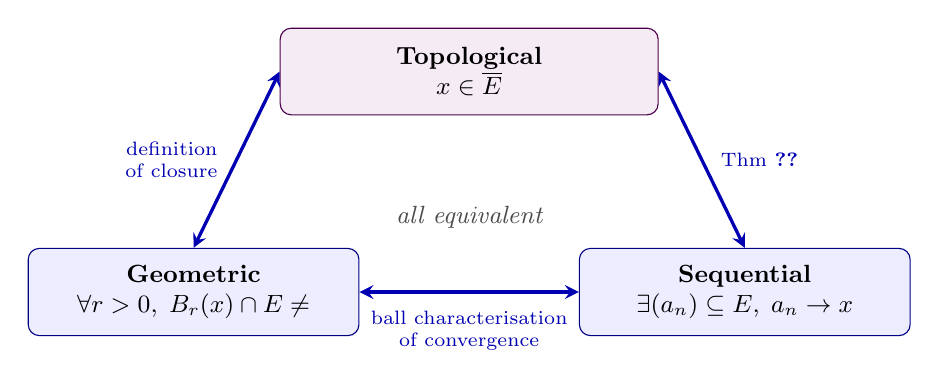
\begin{tikzpicture}[
  box/.style={
    draw=blue!50!black, fill=blue!7, rounded corners=4pt,
    minimum width=4.2cm, minimum height=1.1cm,
    align=center, font=\small, inner sep=6pt
  },
  midbox/.style={
    draw=violet!60!black, fill=violet!8, rounded corners=4pt,
    minimum width=4.8cm, minimum height=1.1cm,
    align=center, font=\small, inner sep=6pt
  },
  arr/.style={->, >=stealth, line width=1.1pt, blue!60!black},
  bidir/.style={<->, >=stealth, line width=1.2pt, blue!70!black},
]

% -- Three nodes in a triangle --
\node[box] (geom) at (0, 0) {
  \textbf{Geometric}\\
  $\forall r > 0,\; B_r(x) \cap E \neq \varnothing$
};

\node[box] (seq) at (7, 0) {
  \textbf{Sequential}\\
  $\exists (a_n) \subseteq E,\; a_n \to x$
};

\node[midbox] (topo) at (3.5, 2.8) {
  \textbf{Topological}\\
  $x \in \overline{E}$
};

% -- Arrows (all bidir since it's an equivalence) --
\draw[bidir] (topo.west) -- (geom.north)
  node[midway, left=3pt, font=\scriptsize, align=right]
  {definition\\of closure};

\draw[bidir] (topo.east) -- (seq.north)
  node[midway, right=3pt, font=\scriptsize, align=left]
  {Thm~\ref{thm:sequential-char-closure}};

\draw[bidir] (geom.east) -- (seq.west)
  node[midway, below=3pt, font=\scriptsize, align=center]
  {ball characterisation\\of convergence};

% -- Central label --
\node[font=\small\itshape, gray!60!black] at (3.5, 0.95) {all equivalent};

\end{tikzpicture}
\caption{The unifying theorem of metric space topology:
$x \in \overline{E}$ if and only if every ball around $x$ meets $E$,
if and only if some sequence in $E$ converges to $x$.
This three-way equivalence links the topological, geometric, and sequential
perspectives and will reappear throughout analysis.}
\label{fig:closure-three-way}
\end{figure}
